\documentclass{article}
\usepackage[utf8]{inputenc}
\usepackage{amsmath}
\usepackage{amsthm}
\usepackage{amsfonts}
\usepackage{amssymb}
\usepackage{amstext}
\usepackage{gensymb}
\usepackage{graphicx}
\usepackage{enumerate}
\pagenumbering{arabic}
\usepackage{fancyhdr}
\usepackage[margin=0.75in]{geometry}
\usepackage{eucal}
\usepackage{parskip} % removes auto indentation for paragraphs
\usepackage{enumitem} % changes the indexing for enumerate
\setlist[enumerate,1]{label = {(\alph*)}}

\usepackage{listings} % import code into latex

\usepackage{subcaption}

\DeclareMathOperator{\tr}{tr}

\def\N{\mathbb{N}}
\def\Z{\mathbb{Z}}
\def\Q{\mathbb{Q}}
\def\R{\mathbb{R}}
\def\C{\mathbb{C}}
\newcommand{\Mod}[1]{\ (\text{mod}\ #1)}
\newcommand{\Problem}[1]{\textbf{\large Problem #1}}
\newcommand{\li}[0]{\liminf_{n\to\infty}}
\newcommand{\ls}[0]{\limsup_{n\to\infty}}
\newcommand{\dl}[2]{\displaystyle\lim_{#1 \to #2}}
\newcommand{\ds}[2]{\displaystyle\sum_{#1}^{#2}}
\newcommand{\ra}{\Rightarrow}

\linespread{1.5}

\usepackage{float}

\pagestyle{fancy}
\fancyhf{}
\rhead{CSE 6643}
\lhead{Alexander Winkles}
\chead{\Large \textbf{Homework 3}}
\cfoot{Page \thepage}

\begin{document}

\Problem{1}

To start, we find the inverse of $A - 1.268 * I$. 
This is found to be 
$$A' = \begin{bmatrix}
 -12242.23178669 & 8962.31366785 & -3280.49548604\\
 8962.31366785 & -6560.41360487 & 2401.32269578\\
 -3280.49548604 & 2401.32269578 & -878.59542305	
 \end{bmatrix}$$.
We choose our initial vector to be $v_0 = \begin{bmatrix}
 1 & 0 & 0	
 \end{bmatrix}^T$. 
Then, our computations are as follows:
\begin{align*}
w_1 &= A' * v_0 = \begin{bmatrix} -12242.23178669 & 8962.31366785 & -3280.49548604 \end{bmatrix}^T\\
v_1 &= w_1 / ||w_1|| = \begin{bmatrix} -0.78866191 & 0.57736494 & -0.21133416 \end{bmatrix}^T \\
\lambda_1 &= 1.26794919 \\
w_2 &= A' * v_1 = \begin{bmatrix} 15522.78828155 & -11363.469684 & 4159.31857608 \end{bmatrix}^T\\
v_2 &= w_2  / ||w_2|| = \begin{bmatrix} 0.78867513 & -0.57735027 & 0.21132487 \end{bmatrix}^T\\
\lambda_2 &= 1.26794919 \\
w_3 &= = A' * v_2 = \begin{bmatrix} -15522.78827785 & 11363.46969452 & -4159.31858333 \end{bmatrix}^T\\
v_3 &= w_3 / ||w_3|| = \begin{bmatrix} -0.78867513 & 0.57735027 & -0.21132487\end{bmatrix}^T\\
\lambda_3 &= 1.26794919
\end{align*}
This computation was very accurate, and in fact converged to machine precision by the first iteration. 
To compare this result, according to Wolfram Alpha the eigenvalue in question is approximately $1.26795$, which is less accurate than our result. 

\Problem{2}

To start, we must first find an appropriate matrix form for the polynomial. 
We will let $A$ be written as follows:
\begin{equation*}
A = \begin{bmatrix}
 0 & & & & & - a_n \\
 1 & 0 & & & & -a_{n-1} \\
 & 1 & 0 & & & - a_{n-2} \\
 & & 1 & \ddots & & \vdots\\
 & & & \ddots & 0 & -a_2 \\
 & & & & 1 & -a_1	
 \end{bmatrix}
\end{equation*}
This matrix form will represent our polynomial - now we must apply the power method to find the eigenvalues of this matrix, which correspond to the roots. 
From here, we may apply the power iteration, which will produce the largest eigenvalue in the absolute value sense, which is identical to the largest root of the polynomial. 

\Problem{3}

Let $A \in \R^{m*n}$ with $m > n$ and $y \in \R$. 
Call $\bar{A} = [A | y]$. 
Recall that the condition number of a matrix is defined as $\kappa = \frac{\sigma_{max}}{\sigma_{min}}$
Now suppose $A = U\Sigma V$ is the singular value decomposition of the original matrix $A$ and let $x$ be the right singular vector corresponding to $\sigma_{max}(A)$. Then, 

$$\sigma_{max}(A) = ||A||_2 = ||Ax||_2 = ||\bar{A}\begin{bmatrix} x \\ 0 \end{bmatrix}||_2 \leq ||\bar{A}||_2||\begin{bmatrix} x \\ 0 \end{bmatrix}||_2 = ||\bar{A}||_2 = \sigma_{max}(\bar{A})$$

Thus we have shown that $\sigma_{max}(A) \leq \sigma_{max}(\bar{A})$. 
By a similar argument, $\sigma_{min}(A) \geq \sigma_{min}(\bar{A})$, or $1 / \sigma_{min}(A) \leq 1 / \sigma_{min}(\bar{A})$.
Combining these results gives us 
$$\kappa(A) = \frac{\sigma_{max}(A)}{\sigma_{min}(A)} \leq \frac{\sigma_{max}(\bar{A})}{\sigma_{min}(\bar{A})} = \kappa(\bar{A}),$$ completing the proof. 

\Problem{4}

My algorithm for the Givens rotation is presented below:

\lstinputlisting[language=Python]{"../../code/givens.py"}

This algorithm, \textit{givensQR}, creates a copy of the input matrix then finds its size.
After that, it loops through various values within the matrix and finds their Givens rotations using \textit{givensrotation}.
With this values, it generates a matrix of the $c$ and $s$ values then multiplies it by the corresponding matrix parts in $R$. 
Notice that this algorithm does not do entire matrix multiplications with the Givens rotation matrix; instead it picks out the appropriate values from $R$ and only multiplies with them (which works because the rest of the Givens matrix is filled with 0s). 
Also notice that this algorithm only generates $R$ and not $Q$.
This was not explicitly asked for in the problem, but the program could easily be altered to generate $Q$ by making a new matrix and continuously multiplying it by the Givens rotation at each step. 

Below is the graph generated when analyzing the algorithm using the method ``problem4'' in \textit{runexperiment3.py}, which generated matrices of the appropriate form and size then performed their QR factorization using the Givens algorithm. 
Based on this, it is clear that the algorithm runs in exponential time. 
In this algorithm, since there are two for loops that could be up to size $n$ and a matrix multiplication that could be up to size $2n$, the total complexity of the algorithm is $O(n^3)$.  

\begin{figure}[H]
\centering
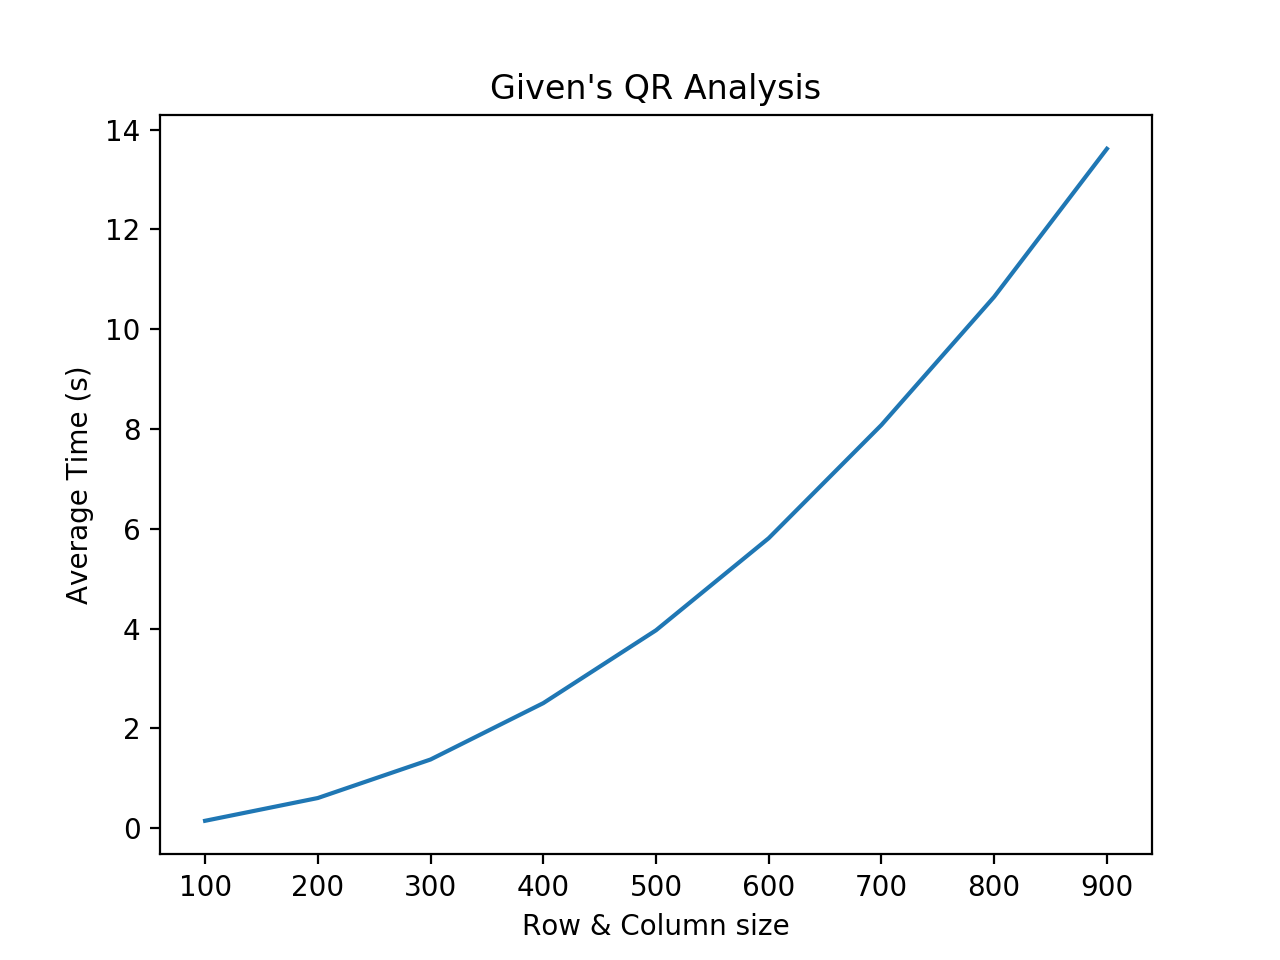
\includegraphics[width=12cm]{givensresult}	
\end{figure}

\Problem{5}

For this problem, I assume that for ``largest and smallest eigenvalues'' this refers to the largest and smallest in the absolute value sense. 
Because of this, I used the power iteration method to compute the largest eigenvalue in the absolute value sense and the inverse iteration method to compute the smallest. 
Here are my codes for them:

\lstinputlisting[language=Python]{"../../code/poweriter.py"}
\lstinputlisting[language=Python]{"../../code/inverseiter.py"}

Then, using the method ``problem5p1" in \textit{runexperiment3.py} I generated the appropriate matrices using the method ``HW3P5'' in \textit{matrixgen.py} and found the average time it took to compute the eigenvalues as well as the average condition number. 
The results for these may be seen below in the figures:
\begin{figure}[H]
\centering
\begin{minipage}[b]{0.4\textwidth}
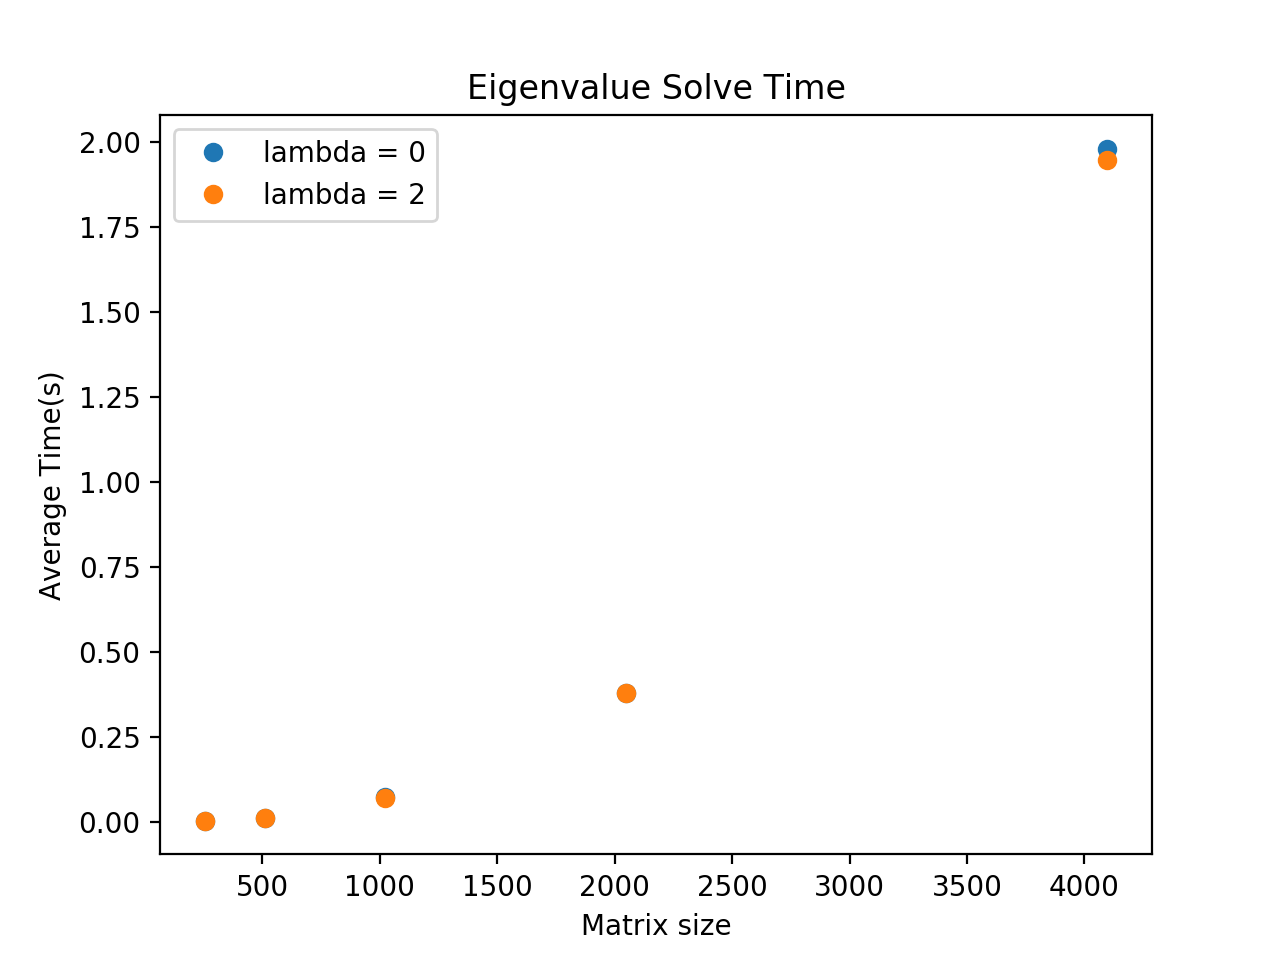
\includegraphics[height=7cm]{eigen}	
\end{minipage}
\hspace{0.6in}
\begin{minipage}[b]{0.4\textwidth}
\centering
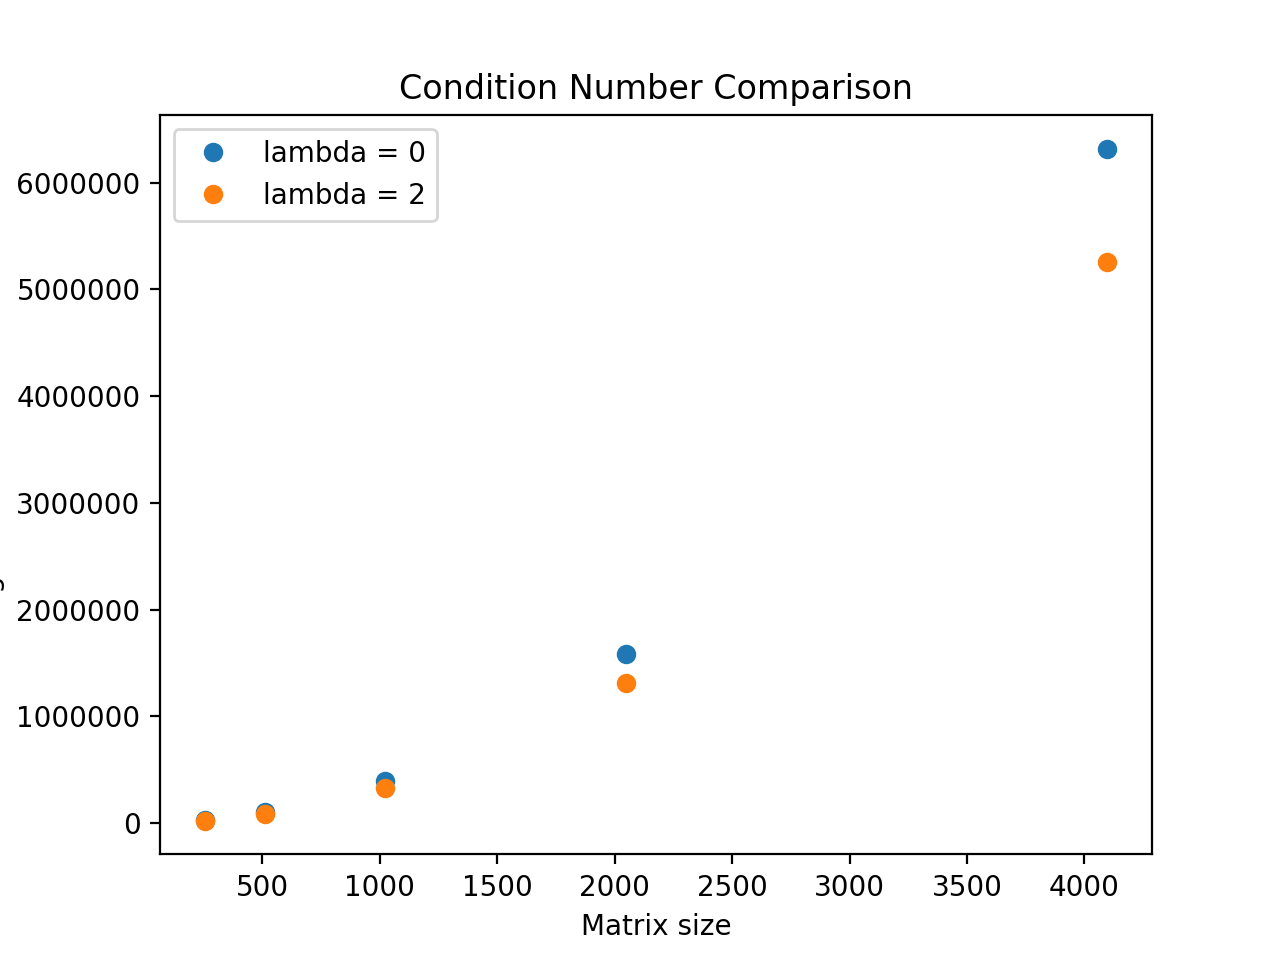
\includegraphics[height=7cm]{condition}	
\end{minipage}
\end{figure}
Note that this was done for $\lambda = 0$ and $\lambda = 2$. 
Each iteration were given 10 steps to run. 
As seen above, the time complexity behaves in an exponential manner. 
This makes sense, as the code for power iteration has complexity of $O(n^2)$ and the complexity for inverse iteration is $O(n^3)$ without processing the matrix ahead of time, giving an overall complexity of $O(n^3)$.
Additionally, as the size of the matrix increases, so too does its condition number in an exponential fashion. 
In other words, the more accurately we try to solve the differential equation using this method (i.e. the bigger the size of the matrix), the more ill-conditioned our problem will become. 
To improve this code in the future, it would be good to add a stopping criteria based on convergence of values.
This could potentially help reduce the time required for computations by adding an additional means to cut off the program. 

For the second part of the problem, I implemented a ``pure'' QR algorithm using Householder QR decomposition.
My code for this can be seen below:

\lstinputlisting[language=Python]{"../../code/pureQR.py"}
\lstinputlisting[language=Python]{"../../code/householder.py"}

This computation is significantly more time consuming than the previous one. 
For this experiment, only five iterations were done per run. 
Unfortunately, my computer was not powerful enough to run the QR algorithm for anything more than a matrix of size 512 without crashing.
Nonetheless, I present my results below:

\begin{figure}[H]
\centering
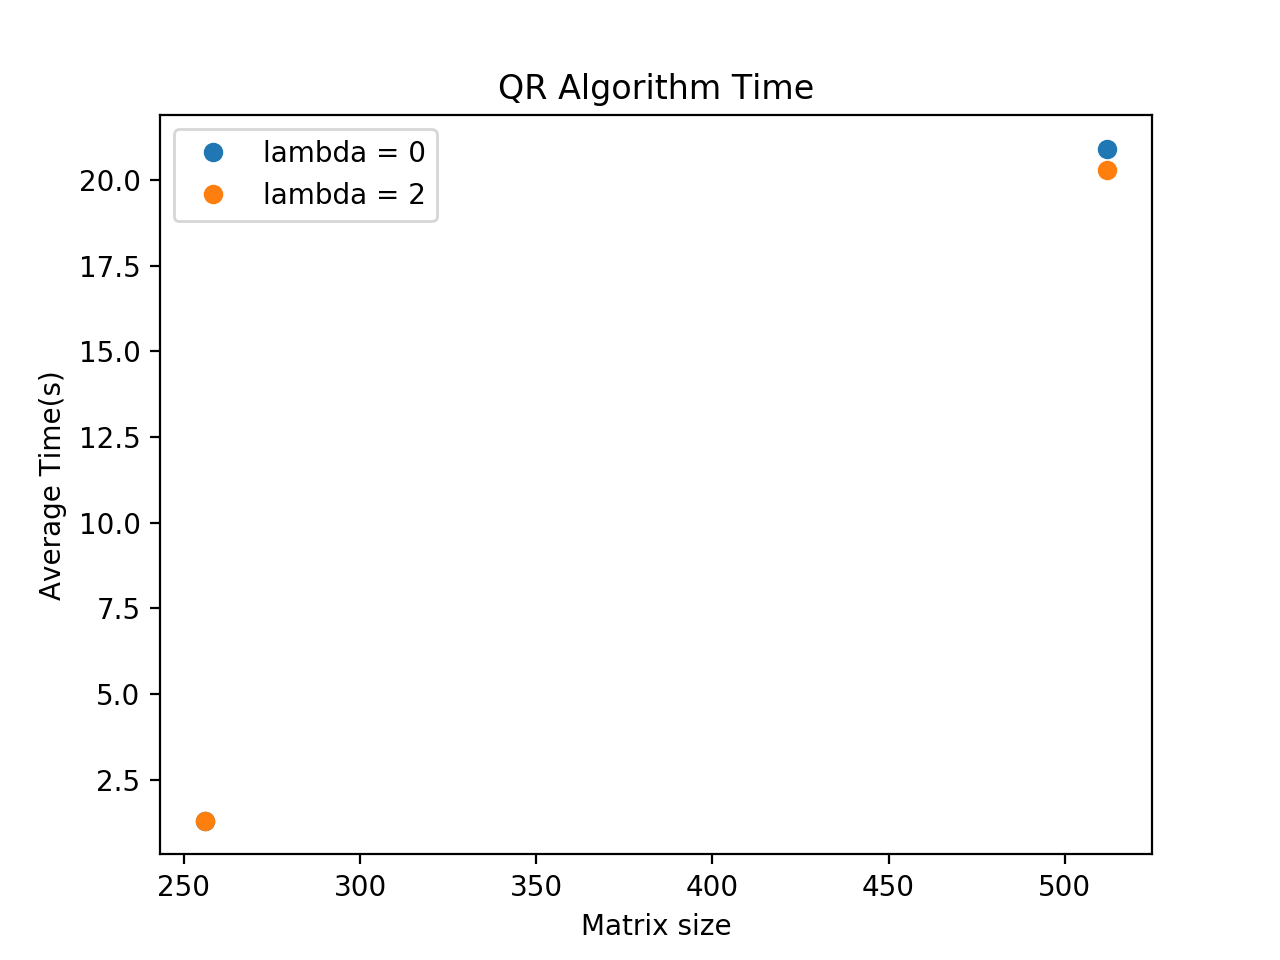
\includegraphics[height=7cm]{QR}	
\end{figure}

Not much is to be gain with this graph (except maybe to see how much more time consuming the algorithm is than the previous ones). 
By analyzing our algorithm, we find that the complexity of this algorithm is $O(n^4)$. 
To improve this in the future, a better QR algorithm (possibly with shifts) may be utilized. 
Additionally, preconditioning the matrix would likewise help improve the time complexity. 

\end{document}